\documentclass[12pt]{article}

\usepackage{amsmath, amssymb}
\usepackage{bm}
\usepackage{upgreek}
\usepackage{tikz}
\usepackage{tikz-3dplot}
\usepackage{geometry}
\usepackage{float}

\geometry{a4paper, margin=1in}

% --- Custom Macros Requested ---
% vectors: boldface, tilde underneath
\newcommand{\vb}[1]{{\underset{\tilde{}}{\mathbf{#1}}}}
% matrices: boldface, underlined
\newcommand{\mb}[1]{\underline{\mathbf{#1}}}
% orthonormal basis {e{}_i}
\newcommand{\bas}[1]{\{ \vb{#1}{}_i \}}
% angular velocity: bold upomega with tilde
\newcommand{\bomega}{\vb{\boldsymbol{\upomega}}}

\title{A rotary self-balancing pendulum through the implementation of PID control}
\author{Philip Tjuatja}
\date{\today}

\begin{document}
\maketitle

\tableofcontents

\section{Dynamics of the inverted pendulum}

This section aims to derive the model for the pendulum system. The following question is posed in a similar fashion to one that I am familiar with when undergoing my university's Intro. to Dynamics and Vibration course (ME2400J). The following derivation is done through the methods introduced in Prof. Parker's Essential Dynamics handout \cite{Parker2026Essential} 

\begin{figure} [H]
\centering
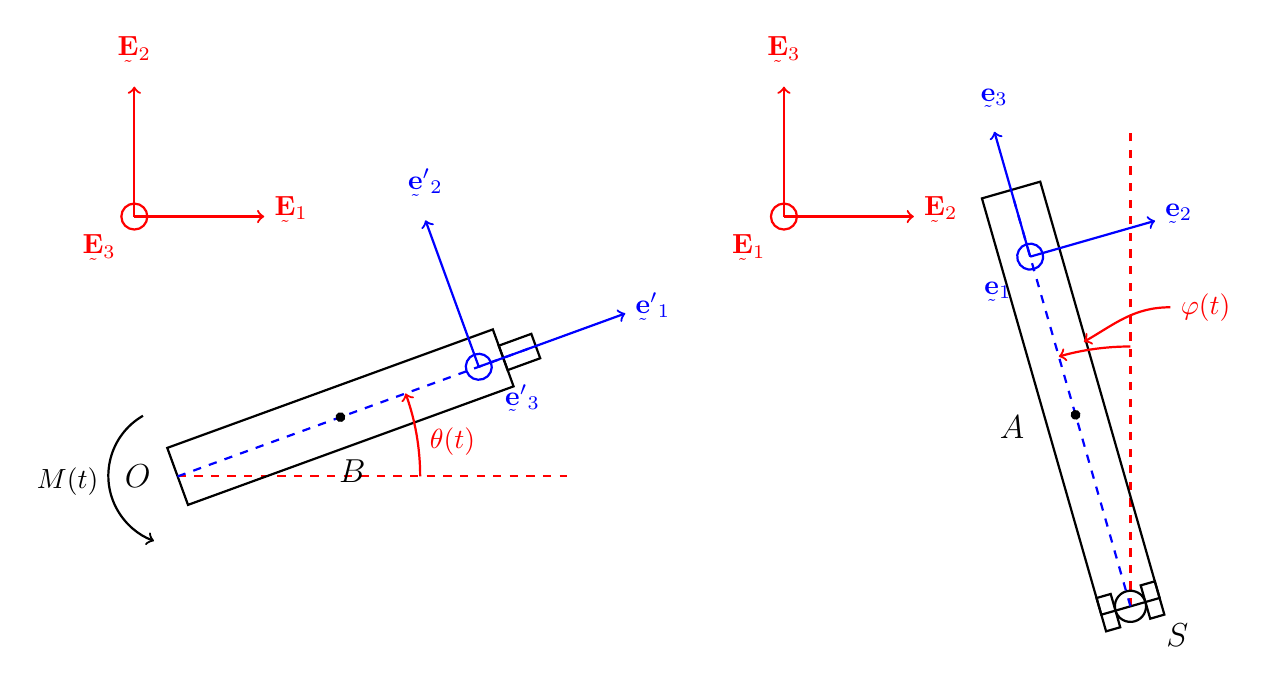
\begin{tikzpicture}[x=1cm, y=1cm, scale=1.1, every node/.style={scale=1}]
    % ==========================================
    % TOP VIEW (Left Side)
    % ==========================================

    % Global Frame E
    \begin{scope}[shift={(-0.5, 3)}]
        \draw[red, thick, ->] (0,0) -- (1.5,0) node[right] {$\vb{E}{}_1$};
        \draw[red, thick, ->] (0,0) -- (0,1.5) node[above] {$\vb{E}{}_2$};
        \draw[red, thick] (0,0) circle (0.15);
        \node[red, anchor=north east] at (-0.1, -0.1) {$\vb{E}{}_3$};
    \end{scope}

    % Arm B & Local Frame
    \begin{scope}[shift={(0,0)}]
        % Base Origin O
        \node[left, font=\large] at (-0.2, 0) {$O$};
        
        % Moment M(t)
        \draw[->, thick] (-0.4, 0.7) arc (120:250:0.8) node[midway, left] {$M(t)$};
        
        % Horizontal Reference Line
        \draw[red, dashed, thick] (0,0) -- (4.5,0);
        
        % Arm B Rotated
        \begin{scope}[rotate=20]
            % Main Arm Rectangle
            \draw[thick] (0, -0.35) rectangle (4, 0.35);
            % End Bracket Rectangle
            \draw[thick] (4, -0.15) rectangle (4.4, 0.15);
            % Centerline
            \draw[blue, dashed, thick] (0,0) -- (4.4,0);
            % Center Dot
            \filldraw[black] (2,0) circle (0.05);
            % Label B
            \node[below, font=\large] at (2, -0.4) {$B$};
            
            % Local Frame e' near the end
            \begin{scope}[shift={(3.7, 0)}] 
                \draw[blue, thick, ->] (0,0) -- (1.8,0) node[right] {$\vb{e}'{}_1$};
                \draw[blue, thick, ->] (0,0) -- (0,1.8) node[above] {$\vb{e}'{}_2$};
                \draw[blue, thick] (0,0) circle (0.15);
                \node[blue, below right] at (0.15, -0.15) {$\vb{e}'{}_3$};
            \end{scope}
        \end{scope}
        
        % Angle theta(t)
        \draw[red, thick, ->] (2.8, 0) arc (0:20:2.8);
        \node[red, right] at (2.8, 0.4) {$\theta(t)$};
    \end{scope}

    % ==========================================
    % FRONT VIEW (Right Side)
    % ==========================================
    \begin{scope}[shift={(7, 0)}]

        % Global Frame E
        \begin{scope}[shift={(0, 3)}]
            \draw[red, thick, ->] (0,0) -- (1.5,0) node[right] {$\vb{E}{}_2$};
            \draw[red, thick, ->] (0,0) -- (0,1.5) node[above] {$\vb{E}{}_3$};
            \draw[red, thick] (0,0) circle (0.15);
            \node[red, anchor=north east] at (-0.1, -0.1) {$\vb{E}{}_1$};
        \end{scope}
        
        % Arm A Pivot Base S
        \coordinate (PivotS) at (4, -1.5);
        
        % Vertical Reference Line
        \draw[red, dashed, thick] (PivotS) -- ++(0, 5.5);
        
        % Arm A Rotated (CCW from vertical)
        \begin{scope}[shift={(PivotS)}, rotate=16] 
            % Side bracket lines (representing the joint)
            \draw[thick] (-0.35, -0.2) rectangle (-0.18, 0.2);
            \draw[thick] (0.18, -0.2) rectangle (0.35, 0.2);
            
            % Main Arm Rectangle A
            \draw[thick] (-0.35, 0) rectangle (0.35, 5);
            % Pivot circle
            \draw[thick] (0,0) circle (0.18);
            % Centerline
            \draw[blue, dashed, thick] (0,0) -- (0, 5);
            % Center Dot
            \filldraw[black] (0, 2.3) circle (0.05);
            % Label A
            \node[left, font=\large] at (-0.5, 2.3) {$A$};
            
            % Label S (red marker at bottom)
            \node[black, right, font=\large] at (0.2, -0.4) {$S$};
            
            % Local Frame e at the top part of the arm
            \begin{scope}[shift={(0, 4.2)}]
                \draw[blue, thick, ->] (0,0) -- (1.5,0) node[right] {$\vb{e}{}_2$};
                \draw[blue, thick, ->] (0,0) -- (0,1.5) node[above] {$\vb{e}{}_3$};
                \draw[blue, thick] (0,0) circle (0.15);
                \node[blue, below left] at (-0.15, -0.15) {$\vb{e}{}_1$};
            \end{scope}
        \end{scope}
        
        % Angle phi(t)
        % Reference vertical is 90 deg, rotated arm is 90 + 16 = 106 deg
        \draw[red, thick, ->] ([shift={(90:3)}]PivotS) arc (90:106:3);
        
        % Pointer and Label for phi(t)
        \draw[red, thick, <-] ([shift={(100:3.1)}]PivotS) to[out=30, in=180] ++(1, 0.4) node[right] {$\varphi(t)$};
        
    \end{scope}
\end{tikzpicture}
\caption{Sketches for the (\textit{left}) top view and (\textit{right}) front view of the rotary inverted pendulum, with bases defined attached.}
\end{figure}

\vspace{0.5cm}

This is a balancing inverted rotary pendulum where a variable moment $M(t)$ is applied about the origin $O$ as shown to keep the pendulum upright. Treatment of these bars are to be rigid bodies; derivations are to neglect dry friction on bearings and viscous drag. Lengths of respective bars are $l{}_A, l{}_B$. Gravity acts in the $-\vb{E}{}_3$ direction. The following are the inertia matrices for both bars about their respective points of reference.
\[
\begin{aligned}
    {}^B\mb{J}^O{}_{\bas{e'}} &= \text{diag}({}^B J{}_1, {}^B J{}_2, {}^B J{}_3) \\
    {}^A\mb{J}^S{}_{\bas{e}} &= \text{diag}({}^A J{}_1, {}^A J{}_2, {}^A J{}_3)
\end{aligned}
\]
Find EoMs for the inverted rotary pendulum.

\subsection{Define origin and bases}
Origin $O$ as shown on the figure. 
\begin{itemize}
    \item $\bas{E}$ : Fixed basis as shown.
    \item $\bas{e'}$ : Rotate $\bas{E}$ by angle $\theta$ about $\vb{E}{}_3$
    \item $\bas{e}$ : Rotate $\bas{e'}$ by angle $\varphi$ about $\vb{e}'{}_1$
\end{itemize}

\begin{center}
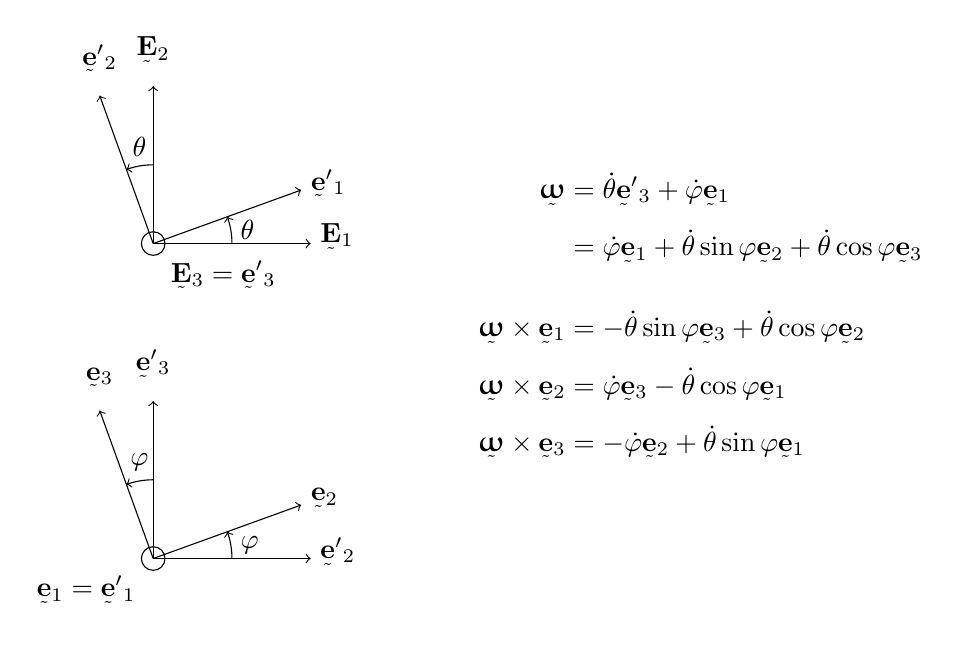
\begin{tikzpicture}[scale=1]
    % Theta rotation
    \draw[->] (0,0) -- (2,0) node[right]{$\vb{E}{}_1$};
    \draw[->] (0,0) -- (0,2) node[above]{$\vb{E}{}_2$};
    \draw[->] (0,0) -- (1.88, 0.68) node[right]{$\vb{e}'{}_1$};
    \draw[->] (0,0) -- (-0.68, 1.88) node[above]{$\vb{e}'{}_2$};
    \draw[->] (1,0) arc (0:20:1) node[midway, right]{$\theta$};
    \draw[->] (0,1) arc (90:110:1) node[midway, above]{$\theta$};
    \draw (0,0) circle (0.15);
    \node[below right] at (0.1,-0.1) {$\vb{E}{}_3 = \vb{e}'{}_3$};

    % Phi rotation
    \begin{scope}[yshift=-4cm]
        \draw[->] (0,0) -- (2,0) node[right]{$\vb{e}'{}_2$};
        \draw[->] (0,0) -- (0,2) node[above]{$\vb{e}'{}_3$};
        \draw[->] (0,0) -- (1.88, 0.68) node[right]{$\vb{e}{}_2$};
        \draw[->] (0,0) -- (-0.68, 1.88) node[above]{$\vb{e}{}_3$};
        \draw[->] (1,0) arc (0:20:1) node[midway, right]{$\varphi$};
        \draw[->] (0,1) arc (90:110:1) node[midway, above]{$\varphi$};
        \draw (0,0) circle (0.15);
        \node[below left] at (-0.1,-0.1) {$\vb{e}{}_1 = \vb{e}'{}_1$};
    \end{scope}
    
    % Math Equations next to it
    \node[anchor=west] at (4, -1) {
        $\begin{aligned}
            \bomega &= \dot{\theta} \vb{e}'{}_3 + \dot{\varphi} \vb{e}{}_1 \\
            &= \dot{\varphi} \vb{e}{}_1 + \dot{\theta} \sin\varphi \vb{e}{}_2 + \dot{\theta} \cos\varphi \vb{e}{}_3 \\[0.3cm]
            \bomega \times \vb{e}{}_1 &= -\dot{\theta}\sin\varphi \vb{e}{}_3 + \dot{\theta}\cos\varphi \vb{e}{}_2 \\
            \bomega \times \vb{e}{}_2 &= \dot{\varphi}\vb{e}{}_3 - \dot{\theta}\cos\varphi \vb{e}{}_1 \\
            \bomega \times \vb{e}{}_3 &= -\dot{\varphi}\vb{e}{}_2 + \dot{\theta}\sin\varphi \vb{e}{}_1
        \end{aligned}$
    };
\end{tikzpicture}
\end{center}

\subsection{Kinematics}
For the center of mass of bar B:
\begin{align*}
    \vb{r}{}_B &= \frac{l{}_B}{2} \vb{e}'{}_1 \\
             &= \frac{l{}_B}{2} \vb{e}{}_1 \\
    \dot{\vb{r}}{}_B &= \frac{l{}_B}{2} \dot{\vb{e}}{}_1 \\
             &= \frac{l{}_B}{2} (-\dot{\theta}\sin\varphi \vb{e}{}_3 + \dot{\theta}\cos\varphi \vb{e}{}_2) \\
    \dot{\vb{r}}{}_B \cdot \dot{\vb{r}}{}_B &= \frac{l{}_B^2}{4}\dot{\theta}^2 \\
    \\
    {}^B\bomega &= \dot{\theta} \vb{e}'{}_3 \\
    \\
    {}^B\bomega \cdot {}^B\mb{J} \cdot {}^B\bomega &= {}^B J{}_3 \dot{\theta}^2 
\end{align*}
For the center of mass of bar A:
\begin{align*}
    \vb{r}{}_A &= \vb{r}{}_B + \frac{l{}_A}{2} \vb{e}{}_3 \\
             &= l{}_B \vb{e}{}_1 + \frac{l{}_A}{2} \vb{e}{}_3 \\
    \dot{\vb{r}}{}_A &= l{}_B (-\dot{\theta}\sin\varphi \vb{e}{}_3 + \dot{\theta}\cos\varphi \vb{e}{}_2) + \frac{l{}_A}{2} (-\dot{\varphi}\vb{e}{}_2 + \dot{\theta}\sin\varphi \vb{e}{}_1) \\
             &= \frac{l{}_A}{2}\dot{\theta}\sin\varphi \vb{e}{}_1 + \left[ -\frac{l{}_A}{2}\dot{\varphi} + l{}_B \dot{\theta}\cos\varphi \right] \vb{e}{}_2 - l{}_B \dot{\theta}\sin\varphi \vb{e}{}_3 \\
    \dot{\vb{r}}{}_A \cdot \dot{\vb{r}}{}_A &= \frac{l{}_A^2}{4}\dot{\theta}^2\sin^2\varphi + \frac{l{}_A^2}{4}\dot{\varphi}^2 + l{}_B^2\dot{\theta}^2\cos^2\varphi + l{}_B^2\dot{\theta}^2\sin^2\varphi - l{}_A l{}_B \dot{\theta}\dot{\varphi}\cos\varphi \\
             &= \frac{l{}_A^2}{4}[\dot{\theta}^2\sin^2\varphi + \dot{\varphi}^2] + l{}_B^2\dot{\theta}^2 - l{}_A l{}_B \dot{\theta}\dot{\varphi}\cos\varphi \\
        {}^A\bomega &= \dot{\varphi} \vb{e}{}_1 + \dot{\theta}\sin\varphi \vb{e}{}_2 + \dot{\theta}\cos\varphi \vb{e}{}_3 \\
        {}^A\bomega \cdot {}^A\mb{J} \cdot {}^A\bomega &= {}^A J{}_1 \dot{\varphi}^2 + {}^A J{}_2 \dot{\theta}^2\sin^2\varphi + {}^A J{}_3 \dot{\theta}^2\cos^2\varphi
\end{align*}


\subsection{Forces and Energy}
Conservative forces such that there exist a respective potential:
\begin{itemize}
    \item Gravity: $-m_A g \vb{E}{}_3$ on Bar A and $-m_B g \vb{E}{}_3$ on Bar B. It should be known that there is no contribution from B since there is no change in $\vb{r}{}_B$ in the $\vb{E}{}_3$ direction.
\end{itemize}

\noindent Constraint forces do not do work and assume no non-conservative forces. Non-conservative moment present acted on origin $O$, that is, the supplied moment by actuator (due to control system for balancing): \(\vb{M} = M(t)\vb{E}{}_3 \) 

\begin{align*}
    T &= \frac{1}{2}m{}_A \dot{\vb{r}}{}_A \cdot \dot{\vb{r}}{}_A + \frac{1}{2}m{}_B \dot{\vb{r}}{}_B \cdot \dot{\vb{r}}{}_B + \frac{1}{2} {}^A\bomega \cdot {}^A\mb{J} \cdot {}^A\bomega + \frac{1}{2} {}^B\bomega \cdot {}^B\mb{J} \cdot {}^B\bomega \\
      &= \frac{1}{2}m{}_A \left( \frac{l{}_A^2}{4} [\dot{\theta}^2\sin^2\varphi + \dot{\varphi}^2] + l{}_B^2\dot{\theta}^2 - l{}_A l{}_B \dot{\theta}\dot{\varphi}\cos\varphi \right) + \frac{1}{2}m{}_B \frac{l{}_B^2}{4} \dot{\theta}^2 \\
      &\quad + \frac{1}{2}\left( {}^A J{}_1 \dot{\varphi}^2 + \left[ {}^A J{}_2 \sin^2\varphi + {}^A J{}_3 \cos^2\varphi + {}^B J{}_3 \right] \dot{\theta}^2 \right) \\
    V &= m{}_A g \vb{E}{}_3 \cdot \vb{r}{}_A = m{}_A g \, \vb{r}{}_A \cdot (\sin\varphi \vb{e}{}_2 + \cos\varphi \vb{e}{}_3) \\
      &= m{}_A g \frac{l{}_A}{2} \cos\varphi
\end{align*}

\subsection{Equations of Motion}
Using Lagrange's equations:
$$ \frac{d}{dt} \frac{\partial T}{\partial \dot{q}} - \frac{\partial T}{\partial q} + \frac{\partial V}{\partial q} = \sum \left( \vb{F}^{nc} \cdot \frac{\partial \vb{r}}{\partial q} + \mb{M}^{nc} \cdot \frac{\partial \bomega}{\partial \dot{q}} \right) $$

\noindent For $\theta$: 
\begin{align*}
    \frac{\partial T}{\partial \dot{\theta}} &= \frac{1}{2}m{}_A \left( \frac{l{}_A^2}{4} 2\dot{\theta}\sin^2\varphi + l{}_B^2 2\dot{\theta} - l{}_A l{}_B \dot{\varphi}\cos\varphi \right) + \frac{1}{2}m{}_B \frac{l{}_B^2}{4} 2\dot{\theta} \\ & \quad + \left({}^A J{}_2 \sin^2\varphi + {}^A J{}_3 \cos^2\varphi + {}^B J{}_3\right) \dot{\theta} \\
    \frac{d}{dt}\frac{\partial T}{\partial \dot{\theta}} &= \frac{l{}_A^2}{4} m{}_A \ddot{\theta}\sin^2\varphi + \frac{l{}_A^2}{4} m{}_A \dot{\theta}\dot{\varphi} 2\sin\varphi\cos\varphi + l{}_B^2 m{}_A \ddot{\theta} + m{}_B \frac{l{}_B^2}{4} \ddot{\theta} \\
    &\quad - \frac{l{}_A l{}_B}{2} m{}_A [\ddot{\varphi}\cos\varphi - \dot{\varphi}^2\sin\varphi] + \left({}^A J{}_2 \sin^2\varphi + {}^A J{}_3 \cos^2\varphi + {}^B J{}_3\right) \ddot{\theta} \\
    &= \left[ m{}_A \left( \frac{l{}_A^2}{4}\sin^2\varphi + l{}_B^2 \right) + m{}_B \frac{l{}_B^2}{4} \right] \ddot{\theta} + \left[ \frac{l{}_A^2}{2} m{}_A \sin\varphi\cos\varphi \right] \dot{\theta}\dot{\varphi}\\ &\quad + \left[ {}^A J{}_2 \sin^2\varphi + {}^A J{}_3 \cos^2\varphi + {}^B J{}_3 \right] \ddot{\theta} \\
    &\quad - m{}_A \left[ \left(\frac{l{}_A l{}_B}{2}\cos\varphi\right)\ddot{\varphi} - \left(\frac{l{}_A l{}_B}{2}\sin\varphi\right)\dot{\varphi}^2 \right] \\
    \frac{\partial T}{\partial \theta} &= 0 \quad ; \quad \frac{\partial V}{\partial \theta} = 0 \quad ; \quad (M\sin\varphi \vb{e}{}_2 + M\cos\varphi \vb{e}{}_3) \cdot (\sin\varphi \vb{e}{}_2 + \cos\varphi \vb{e}{}_3) = M \\
    \\
    &\Rightarrow \left[ m{}_A \left(\frac{l{}_A^2}{4}\sin^2\varphi + l{}_B^2\right) + m{}_B \frac{l{}_B^2}{4} \right] \ddot{\theta} + \left[ \frac{l{}_A^2}{2} m{}_A \sin\varphi \cos\varphi \right] \dot{\theta}\dot{\varphi}\\ &\quad + \left[ {}^A J{}_2 \sin^2\varphi + {}^A J{}_3 \cos^2\varphi + {}^B J{}_3 \right]\ddot{\theta} \\
    &\quad - m{}_A \left[ \left(\frac{l{}_A l{}_B}{2}\cos\varphi\right)\ddot{\varphi} - \left(\frac{l{}_A l{}_B}{2}\sin\varphi\right)\dot{\varphi}^2 \right] = M(t)
\end{align*}

\noindent For $\varphi$: 
\begin{align*}
    \frac{\partial T}{\partial \dot{\varphi}} &= m{}_A \frac{l{}_A^2}{4} \dot{\varphi} + {}^A J{}_1 \dot{\varphi} - m{}_A \frac{l{}_A l{}_B}{2} \dot{\theta} \cos\varphi\\
    \frac{d}{dt}\frac{\partial T}{\partial \dot{\varphi}} &= \left[ m{}_A \frac{l{}_A^2}{4} + {}^A J{}_1 \right] \ddot{\varphi} - \left[ \left( m{}_A \frac{l{}_A l{}_B}{2} \ddot{\theta} \cos\varphi \right) - \left( m{}_A \frac{l{}_A l{}_B}{2} \dot{\theta}\dot{\varphi} \sin\varphi \right) \right] \\
    \frac{\partial T}{\partial \varphi} &= \frac{1}{2} m{}_A \frac{l{}_A^2}{4} \dot{\theta}^2 \cdot 2\sin\varphi\cos\varphi + m{}_A \frac{l{}_A l{}_B}{2} \dot{\theta}\dot{\varphi}\sin\varphi \\
    &\quad + {}^A J{}_2 \dot{\theta}^2 \sin\varphi\cos\varphi - {}^A J{}_3 \dot{\theta}^2 \cos\varphi\sin\varphi \\
    \frac{\partial V}{\partial \varphi} &= -m{}_A g \frac{l{}_A}{2} \sin\varphi \quad; \quad(M\sin\varphi \vb{e}{}_2 + M\cos\varphi \vb{e}{}_3) \cdot (\vb{e}{}_1) = 0\\
    \\
    &\Rightarrow \left[ m{}_A \frac{l{}_A^2}{4} + {}^A J{}_1 \right] \ddot{\varphi} - \left[ m{}_A \frac{l{}_A^2}{4} + {}^A J{}_2 - {}^A J{}_3 \right] \dot{\theta}^2\sin\varphi\cos\varphi \\ &\quad - \left( m{}_A \frac{l{}_A l{}_B}{2} \right) \ddot{\theta} \cos\varphi - m{}_A g \frac{l{}_A}{2} \sin\varphi = 0
\end{align*}

\vspace{0.5cm}
Hence:
\begin{equation}
    \begin{aligned}
    &\left[ m{}_A \left(\frac{l{}_A^2}{4}\sin^2\varphi + l{}_B^2\right) + m{}_B \frac{l{}_B^2}{4} \right] \ddot{\theta} + \left[ \frac{l{}_A^2}{2} m{}_A \sin\varphi\cos\varphi \right] \dot{\theta}\dot{\varphi} \\
    &\quad + \left[ {}^A J{}_2 \sin^2\varphi + {}^A J{}_3 \cos^2\varphi + {}^B J{}_3 \right]\ddot{\theta} \\
    &\quad - m{}_A \left[ \left(\frac{l{}_A l{}_B}{2}\cos\varphi\right)\ddot{\varphi} - \left(\frac{l{}_A l{}_B}{2}\sin\varphi\right)\dot{\varphi}^2 \right] & &= M(t) \\
    \\
    &\left[ m{}_A \frac{l{}_A^2}{4} + {}^A J{}_1 \right] \ddot{\varphi} - \left[ m{}_A \frac{l{}_A^2}{4} + {}^A J{}_2 - {}^A J{}_3 \right] \dot{\theta}^2\sin\varphi\cos\varphi \\ &\quad - \left(m{}_A \frac{l{}_A l{}_B}{2}\right)\ddot{\theta}\cos\varphi & &=  m{}_A g \frac{l{}_A}{2} \sin\varphi
\end{aligned} 
\label{eq:eom}
\end{equation}
are the EoMs. The model is complete since there are 2 unknowns $\theta, \varphi$ and 2 equations obtained in the model. Rewriting (\ref{eq:eom}) in matrix form yields the equation 
$$ \mb{M} \ddot{\vb{q}} + \mb{C} \dot{\vb{q}} = \vb{\boldsymbol{\uptau}}$$
where, by denoting the following terms for simplicity: 
\begin{itemize}
    \item[] $J{}_\theta = m{}_A l{}_B^2 + m{}_B \frac{l{}_B^2}{4} + {}^B J{}_3 + {}^A J{}_3 \quad \text{(constant base inertia)}$
    \item[] $J{}_\varphi = m{}_A \frac{l{}_A^2}{4} + {}^A J{}_1 \quad \text{(constant pendulum inertia)}$
    \item[] $B = m{}_A \frac{l{}_A^2}{4} + {}^A J{}_2 - {}^A J{}_3 \quad \text{(inertia variation amplitude)}$
    \item[] $L = \frac{l{}_A l{}_B}{2} m{}_A \quad \text{(coupling magnitude)}$
\end{itemize}
we obtain the mass matrix $\mb{M}(\vb{q})$, Christoffel matrix $\mb{C}(\vb{q}, \dot{\vb{q}})$ and moment vector $\vb{\boldsymbol{\uptau}}(\vb{q}, t)$ of the system, given in terms of the modal coordinate $\vb{q}$:

$$\mb{M}, \mb{C} \in \mathcal{M}{}_2(\mathbb{R}), \quad \vb{q} = \begin{bmatrix} \theta \\ \varphi \end{bmatrix} ; \quad \boldsymbol{\uptau} = \begin{bmatrix} M(t) \\  m{}_A g \frac{l{}_A}{2} \sin\varphi \end{bmatrix} $$

\begin{align*}
    \mb{M} &= \begin{bmatrix} J{}_\theta + B\sin^2\varphi & -L\cos\varphi \\ -L\cos\varphi & J{}_\varphi \end{bmatrix} \\
    \\
    \mb{C} &= \begin{bmatrix} B \dot{\varphi} \sin\varphi\cos\varphi & B \dot{\theta} \sin\varphi\cos\varphi + L \dot{\varphi} \sin\varphi \\ -B \dot{\theta} \sin\varphi\cos\varphi & 0 \end{bmatrix}
\end{align*}


\newpage
% ==========================================
% SECTION: SYSTEM BLUEPRINT AND TIKZ SETUP
% ==========================================
\section{Blueprint for Implementation and Control}

This section outlines the detailed procedure for developing a physical Rotary Inverted Pendulum (Furuta Pendulum) based on the derived mathematical model, focusing specifically on transitioning the pendulum from its stable downward position ($\varphi = \pi, \theta = 0$) to its unstable upright position ($\varphi = 0, \theta = 0$) and maintaining balance using a cascaded PID control scheme.

\subsection{Physical System Overview}

\begin{center}
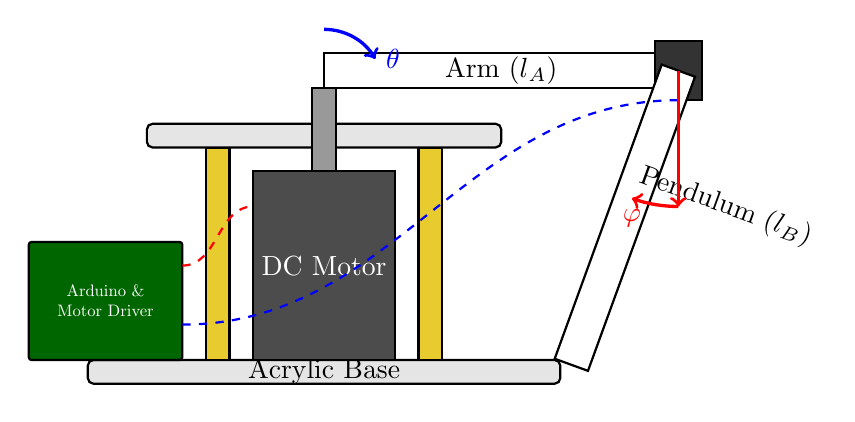
\begin{tikzpicture}[scale=1.5, thick]
    % Base
    \draw[rounded corners=2pt, fill=gray!20] (-2, 0) rectangle (2, 0.2);
    \node at (0, 0.1) {Acrylic Base};
    
    % Standoffs
    \filldraw[fill=yellow!60!brown] (-1, 0.2) rectangle (-0.8, 2);
    \filldraw[fill=yellow!60!brown] (0.8, 0.2) rectangle (1, 2);
    
    % Mid Plate
    \draw[rounded corners=2pt, fill=gray!20] (-1.5, 2) rectangle (1.5, 2.2);
    
    % DC Motor
    \filldraw[fill=black!70] (-0.6, 0.2) rectangle (0.6, 1.8);
    \node[white] at (0, 1) {DC Motor};
    
    % Motor Shaft
    \filldraw[fill=gray!80] (-0.1, 1.8) rectangle (0.1, 2.5);
    
    % Rotary Arm (Link A)
    \draw[fill=white] (0, 2.5) rectangle (3, 2.8);
    \node at (1.5, 2.65) {Arm ($l{}{}_A$)};
    
    % Encoder Joint
    \filldraw[fill=black!80] (2.8, 2.4) rectangle (3.2, 2.9);
    
    % Pendulum Link (Link B) - downward initial state
    \draw[fill=white, rotate around={-20:(3, 2.65)}] (2.85, 2.65) rectangle (3.15, 0);
    \node[rotate=-20] at (3.4, 1.5) {Pendulum ($l{}{}_B$)};
    
    % Electronics Board
    \draw[fill=green!40!black, rounded corners=1pt] (-2.5, 0.2) rectangle (-1.2, 1.2);
    \node[white, align=center, scale=0.6] at (-1.85, 0.7) {Arduino \& \\ Motor Driver};
    
    % Wires
    \draw[red, dashed] (-1.2, 1.0) to[out=0, in=180] (-0.6, 1.5);
    \draw[blue, dashed] (-1.2, 0.5) to[out=0, in=180] (3.0, 2.4);

    % Angles
    \draw[->, blue, very thick] (0, 3) arc (90:30:0.5) node[right]{$\theta$};
    \draw[->, red, very thick] (3, 2.65) -- (3, 1.5);
    \draw[->, red, very thick] (3, 1.5) arc (-90:-110:1.15) node[below]{$\varphi$};

\end{tikzpicture}
\end{center}


\subsection{Physical Setup and Components}

A robust physical setup is paramount because control algorithms are highly sensitive to mechanical backlash, sensor noise, and friction.

\begin{itemize}
    \item \textbf{Microcontroller:} An \textbf{Arduino Teensy (4.0 or 4.1)} or an \textbf{ESP32} is highly recommended over a standard Arduino Uno. Balancing inverted pendulums requires fast floating-point arithmetic and high-speed hardware interrupts (ideally a control loop running at $200\text{Hz}$ to $500\text{Hz}$).
    \item \textbf{Actuation:} A high-torque, low-backlash DC motor (e.g., NEMA-17 sized DC servo or a planetary gear motor with a low gear ratio). 
    \item \textbf{Motor Driver:} A fast-switching H-bridge motor driver like the \textbf{BTS7960} or \textbf{Cytron MD10C} to handle high transient currents during swing-up and direction reversals.
    \item \textbf{Sensors (Encoders):} 
        \begin{itemize}
            \item \textbf{Arm Encoder (for $\theta$):} Mounted on the base motor shaft. Needs at least $1000$ PPR (Pulses Per Revolution) to detect minute base movements.
            \item \textbf{Pendulum Encoder (for $\varphi$):} Mounted at the joint $S$ between the arm $B$ and pendulum $A$. This is the most critical sensor and should be an optical encoder with $2000+$ PPR to accurately calculate the velocity $\dot{\varphi}$.
        \end{itemize}
    \item \textbf{Mechanical Links:} The arm (Link $B$) and pendulum (Link $A$) should be made of lightweight, rigid materials (e.g., carbon fiber, 3D printed PETG, or aluminum). Minimizing $J_\varphi$ and $J_\theta$ improves the dynamic response.
\end{itemize}

\subsection{Control Theory: Swing-Up and Balance}

Because the system is severely nonlinear, a single PID controller cannot operate across the entire state space. A Finite State Machine (FSM) is used to switch between an \textbf{Energy-Pumping Controller} (State 1) and a \textbf{Balancing Controller} (State 2).

\subsubsection{State 1: Swing-Up Control (Energy Based)}
The pendulum starts at rest downwards ($\varphi = \pi$). The goal is to rock the base arm back and forth to pump kinetic energy into the pendulum until it reaches the upright position ($\varphi = 0$).

From the derived model, the total mechanical energy of the pendulum $A$ is:
$$ E = \frac{1}{2} J{}_\varphi \dot{\varphi}^2 + m{}_A g \frac{l{}_A}{2} (\cos\varphi - 1) $$
\textit{(Note: We shift the datum so $E=0$ when the pendulum is perfectly upright at rest ($\varphi=0, \dot{\varphi}=0$)).}

We define the reference energy $E_{ref} = 0$. The energy error is $\tilde{E} = E - E_{ref} = E$. We apply a nonlinear control law based on Lyapunov design to drive $\tilde{E} \to 0$:
$$ M(t)_{swing} = k_E \cdot E \cdot \text{sgn}(\dot{\varphi}\cos\varphi) $$
where $k_E$ is a tunable positive gain. 
\textbf{Physical Meaning:} If the pendulum lacks energy ($E < 0$), the arm accelerates in the direction of the pendulum's swing to add energy. As it approaches the top, the energy error nears zero, and the arm slows down to gently "toss" the pendulum into the balancing zone.

\subsubsection{State 2: Balancing Control (Dual PID)}
Once the pendulum is near the vertical equilibrium ($|\varphi| \le \pm 0.2$ radians), the control switches to balancing mode. 

Although State-Space (LQR) is standard, the system can be stabilized using two superimposed PID loops (often called a Cascaded or Dual PID). The system has 1 input ($M(t)$) and 2 tracked variables ($\varphi$ and $\theta$).
$$ M(t)_{bal} = \text{PID}_{\text{pend}} + \text{PD}_{\text{arm}} $$
$$ M(t)_{bal} = \left[ K_{p,\varphi} \varphi + K_{d,\varphi} \dot{\varphi} + K_{i,\varphi} \int \varphi \, dt \right] + \left[ K_{p,\theta} (\theta - \theta_{ref}) + K_{d,\theta} \dot{\theta} \right] $$

\begin{itemize}
    \item \textbf{Inner Loop ($\varphi$):} This is highly aggressive. If the pendulum falls slightly to the right, the arm must dart to the right to catch it. (Hence $K_{p,\varphi} > 0, K_{d,\varphi} > 0$).
    \item \textbf{Outer Loop ($\theta$):} Without this loop, the pendulum might balance, but the arm will slowly drift in a circle until it rips out its wires. This loop gently "drags" the arm back to the center ($\theta=0$) without knocking the pendulum over.
\end{itemize}

\subsection{Software Implementation Steps}

\textbf{Step 3.1: Hardware Interrupts for Encoders}\\
Do not use standard `digitalRead()` for encoders. Use hardware interrupts (e.g., `attachInterrupt()` in Arduino) to track the quadrature pulses. 
$$ \theta = \left( \frac{\text{ticks}_\theta}{\text{PPR}_\theta} \right) \cdot 2\pi, \quad \varphi = \left( \frac{\text{ticks}_\varphi}{\text{PPR}_\varphi} \right) \cdot 2\pi $$

\textbf{Step 3.2: Velocity Calculation and Filtering}\\
Derivatives are extremely noisy. Calculate $\dot{\varphi}$ and $\dot{\theta}$ inside a fixed time-step loop ($\Delta t = 0.005$ s).
$$ \dot{\varphi}_{raw} = \frac{\varphi_{new} - \varphi_{old}}{\Delta t} $$
Apply a first-order Low-Pass Filter (LPF) to smooth the velocity:
$$ \dot{\varphi}_{filt} = \alpha \dot{\varphi}_{raw} + (1 - \alpha)\dot{\varphi}_{old\_filt} $$
where $\alpha \approx 0.1$ to $0.3$ (tuned to minimize delay while removing high-frequency noise).

\textbf{Step 3.3: The Main Control Loop}\\
Set up a hardware timer to fire every $5\text{ms}$ ($200\text{Hz}$).
\begin{verbatim}
void controlLoop() {
    // 1. Read Sensors & Filter velocities
    // 2. Check State
    if (abs(phi) < 0.2) { 
        // Inside capture zone -> BALANCE
        torque = kp_phi * phi + kd_phi * dPhi_filt + 
                 kp_theta * theta + kd_theta * dTheta_filt;
    } else {
        // Outside capture zone -> SWING UP
        energy = 0.5 * J_phi * sq(dPhi_filt) + m_A * g * L_A/2 * (cos(phi) - 1);
        torque = k_E * energy * sign(dPhi_filt * cos(phi));
        
        // Add safety limit to prevent the arm spinning out of control
        torque = constrain(torque, -MAX_TORQUE, MAX_TORQUE);
    }
    // 3. Output to Motor (Convert Torque to PWM)
    setMotorPWM(torque);
}
\end{verbatim}

\subsection{Step-by-Step Tuning Procedure}

Tuning a MIMO nonlinear system manually is dangerous if done haphazardly. Follow this strict phased approach:

\textbf{Phase 1: Sensor \& Direction Verification}
\begin{itemize}
    \item Print $\varphi$ and $\theta$ to the serial monitor. Verify that moving the pendulum upward to the vertical yields $\varphi \to 0$.
    \item Apply a positive PWM to the motor. Verify that the arm $\theta$ moves in the direction that mathematically corresponds to a positive torque in your coordinate frame. \textit{(If the motor drives opposite to the math, the system will immediately violently crash).}
\end{itemize}

\textbf{Phase 2: Tune Inner Loop (Pendulum $\varphi$)}
\begin{itemize}
    \item Keep the swing-up logic disabled. Manually hold the pendulum upright.
    \item Set $K_{i,\varphi} = 0, K_{p,\theta} = 0, K_{d,\theta} = 0$. 
    \item Increase $K_{p,\varphi}$ until the arm actively fights your hand to keep the pendulum up. It will vibrate and oscillate wildly.
    \item Increase $K_{d,\varphi}$ (Damping). The high-frequency oscillations should smooth out. The arm should now feel like a smooth, stiff spring pushing against your hand.
    \item Let go. The pendulum should balance for a few seconds before drifting to one side and falling.
\end{itemize}

\textbf{Phase 3: Tune Outer Loop (Arm $\theta$)}
\begin{itemize}
    \item With the pendulum balancing (briefly), introduce a very small $K_{p,\theta}$. Notice that to move the arm left, the motor must first jerk right to unbalance the pendulum leftward, then chase it left. Therefore, $K_{p,\theta}$ and $K_{p,\varphi}$ must act cooperatively. 
    \item Introduce a small $K_{d,\theta}$ to dampen the arm's base swinging. 
    \item \textit{Note:} $K_{p,\varphi}$ and $K_{d,\varphi}$ will always be an order of magnitude larger than the arm gains.
\end{itemize}

\textbf{Phase 4: Tune Swing-Up ($k_E$)}
\begin{itemize}
    \item Let the pendulum hang down. Enable the swing-up state.
    \item Increase $k_E$ gradually. The arm will begin to rock back and forth. 
    \item If $k_E$ is too low, it will never reach the top. If $k_E$ is too high, it will overshoot $\varphi = 0$ with too much velocity for the PID to "catch" it.
    \item Tune $k_E$ until the pendulum enters the $|\varphi| < 0.2$ capture zone with near-zero velocity, allowing the PID controller to seamlessly take over.
\end{itemize}

\bibliography{main}
\bibliographystyle{plain}

\end{document}